\documentclass[ignorenonframetext,compress]{beamer}

\usepackage{graphicx}
\usepackage{amsmath}
\usepackage{listings}
\usetheme[framenumber,darktitle]{UniversiteitAntwerpen}
\usepackage[dutch]{babel}
\usepackage{color}


\title{Lindenmayer Systems}
\subtitle{An efficient implementation}
\author{Wouter ibens}
\begin{document}

\frame<presentation>{\titlepage}
\only<article>{\maketitle}

\begin{frame}[fragile]
	\frametitle{}
\begin{center}
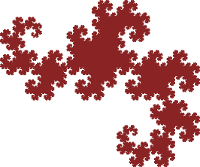
\includegraphics[scale=0.5]{dragon.png}
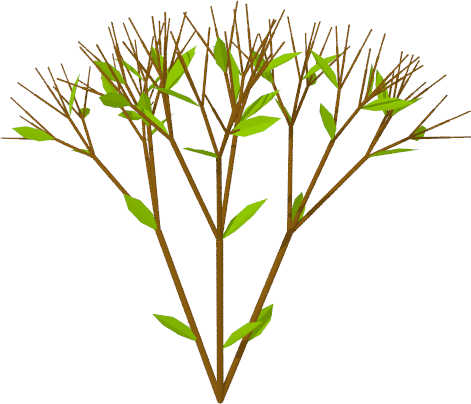
\includegraphics[scale=0.3]{plant6.png}
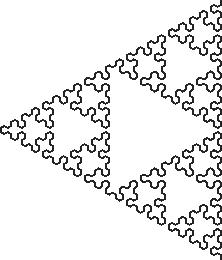
\includegraphics[scale=0.4]{triangle.png}
\end{center}
\end{frame}


\begin{frame}[fragile]
	\frametitle{Inhoud}
\tableofcontents
\end{frame}

\section{Wat zijn L-Systemen}
\subsection{Turtle Graphics}

\begin{frame}[fragile]
	\frametitle{Turtle graphics}
\begin{itemize}
\item Een alfabet, verzameling acties en een mapping hiertussen
\item Een hoek $\sigma$
\item Een pen met locatie en richting
\end{itemize}
\end{frame}

\begin{frame}[fragile]
	\frametitle{Turtle graphics - Voorbeeld}
\begin{itemize}
\item Alfabet = \{F, f, +, -\}
\item $\sigma = 60^{\circ}$
\item Acties = \{Teken lijn van lengte 1, beweeg vooruit met lengte 1, draai $\sigma$ linksom, draai $\sigma$ rechtsom\}
\pause
\item Mapping: \begin{itemize}
	\item[F] $\rightarrow$ Teken lijn
	\item[f] $\rightarrow$ Beweeg vooruit (zonder te tekenen)
	\item[+] $\rightarrow$ Draai $\sigma$ linksom
	\item[-] $\rightarrow$ Draai $\sigma$ rechtssom	
	\end{itemize}
\end{itemize}
\end{frame}

\begin{frame}[fragile]
	\frametitle{Turtle graphics - Voorbeeld}
\begin{center}
\onslide<1>{$F+F--F+F--F+F--F+F--F+F--F+F$} \\
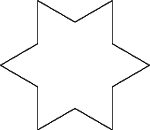
\includegraphics[]{koch2.png}
\end{center}
\end{frame}

\subsection{De basis}
\begin{frame}[fragile]
	\frametitle{L-Systemen}
\begin{itemize}
\item De strings voor turtle graphics dynamisch opbouwen
\item We voegen een beginstring (axiom) een een formele grammar toe.
\pause
\item Voorbeeld:
	\begin{itemize}
	\item Axiom = $F--F--F$
	\item Grammar: $F \rightarrow F+F--F+F$
	\end{itemize}
\end{itemize}
\end{frame}

\begin{frame}[fragile]
	\frametitle{L-Systemen - Voorbeeld}
\begin{center}
\begin{tabular}{c c c c}
Iteratie 0 & Iteratie 1 & Iteratie 2 & Iteratie 3 \\
(Axiom) \\
\onslide<1->{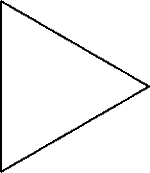
\includegraphics[scale=0.40]{koch1.png}} &
\onslide<2->{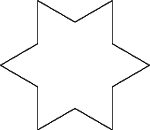
\includegraphics[scale=0.50]{koch2.png}} &
\onslide<3->{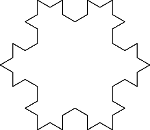
\includegraphics[scale=0.50]{koch3.png}} &
\onslide<4->{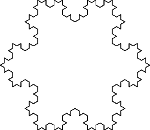
\includegraphics[scale=0.50]{koch4.png}} \\
\end{tabular}
\onslide<1,2>{$F--F--F$}
\onslide<2>{$\underline{F+F--F+F}--\underline{F+F--F+F}--\underline{F+F--F+F}$}
\end{center}
\end{frame}

\subsection{Uitbreidingen}
\begin{frame}[fragile]
	\frametitle{L-Systemen - Uitbreidingen}
\begin{description}
\item[Brackets*] Een stackimplementatie om deelbomen te genereren en verder te gaan op de originele locatie.
\item[3D] Een derde dimensie
\item[Polygonen*] Lijnentekening vullen
\item[Stijlen] Dikte, lengte en kleur aanpassen
\item[Parameters] Acties verfijnen dankzij parameters 
\item[Stochastisch] Verschillende productieregels per symbool, met bepaalde kans 
\end{description}
\end{frame}

\begin{frame}[fragile]
	\frametitle{Brackets}
\begin{itemize}
\item Brackets pushen/poppen de huidige staat op een stack
\item Hierdoor kan een boom takken (met takken, met takken ...) hebben
\pause
\item \textcolor{red}{F}[+F]\textcolor{blue}{F}[+F]\textcolor{green}{F}[+F]\textcolor{yellow}{F}[+F] ($\sigma = 90^{\circ}$)
\item 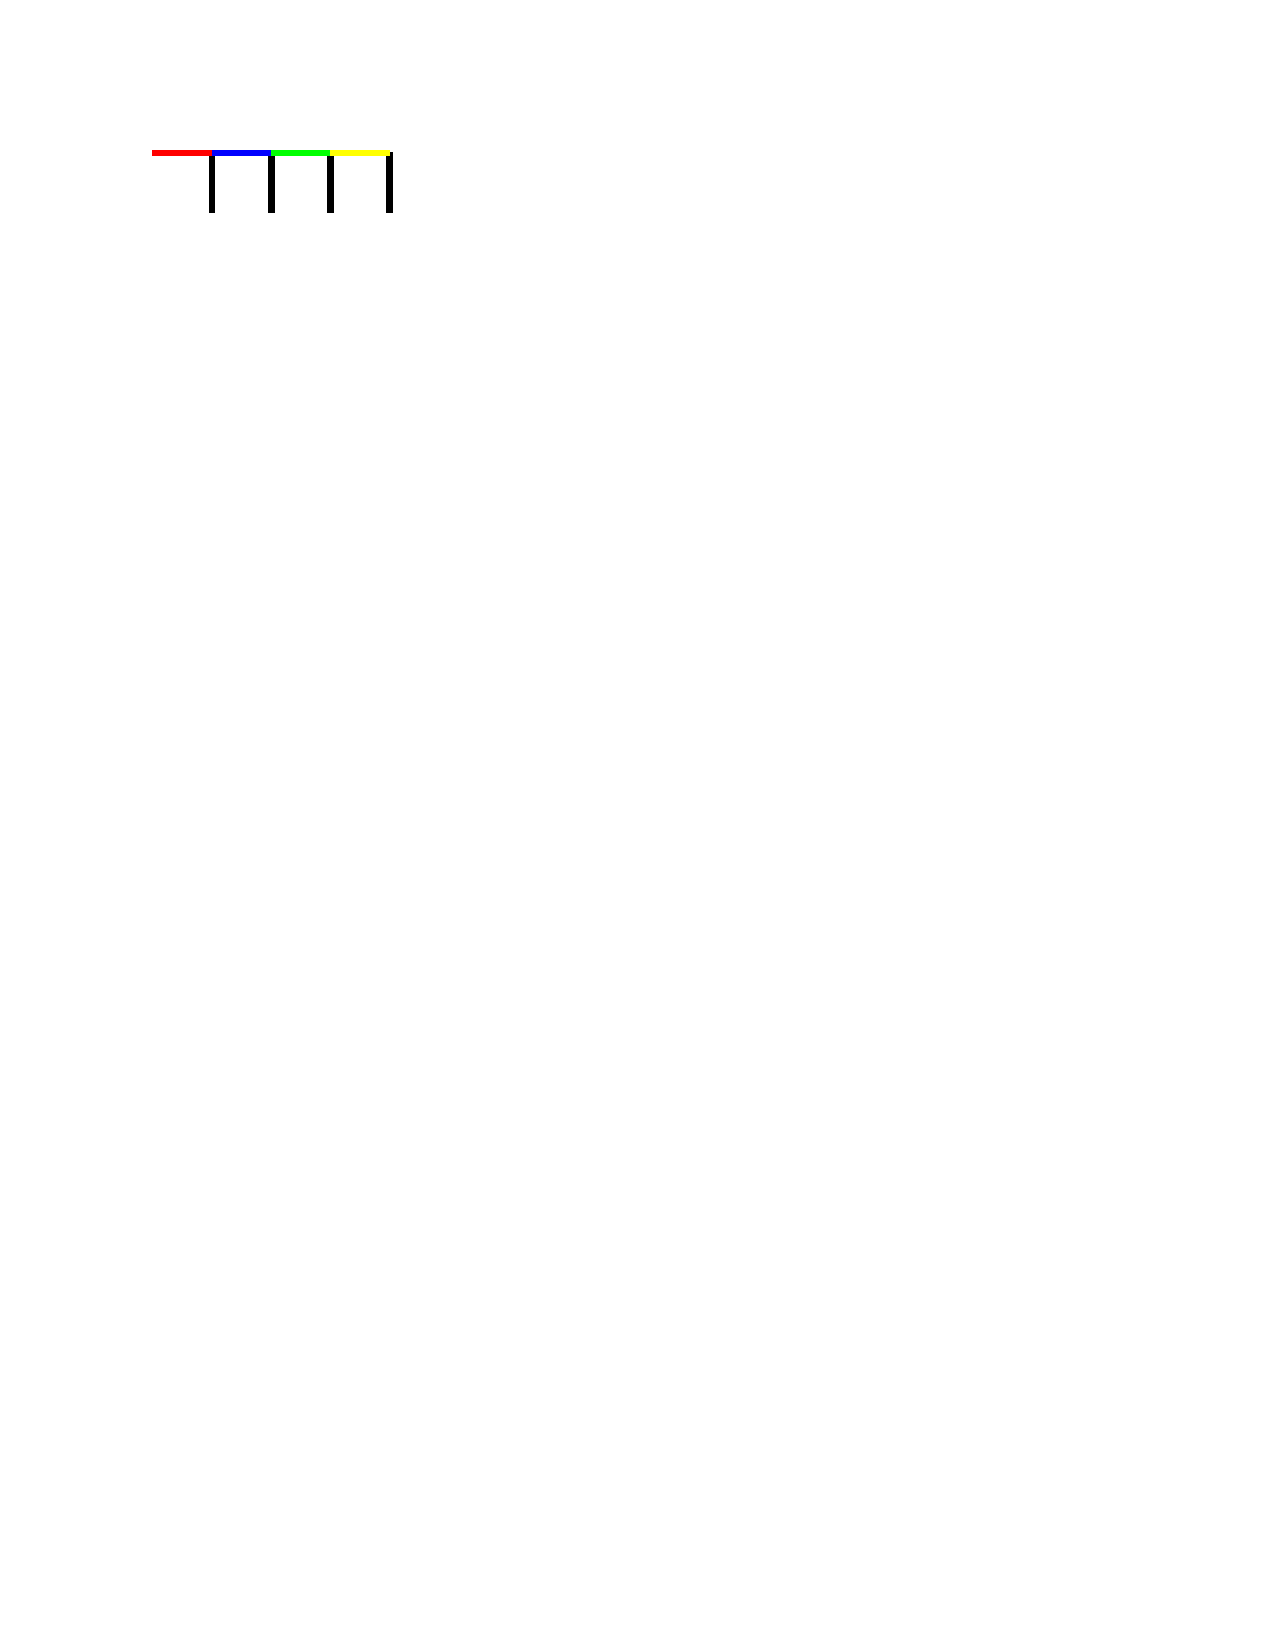
\includegraphics[trim = 24mm 00mm 0mm 24mm, clip]{brackets.pdf}
\end{itemize}
\end{frame}

\begin{frame}[fragile]
	\frametitle{}
\begin{center}
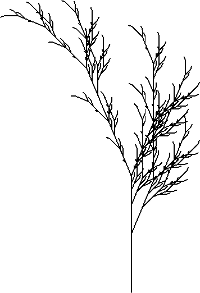
\includegraphics[width=0.38\textwidth]{tree.png}
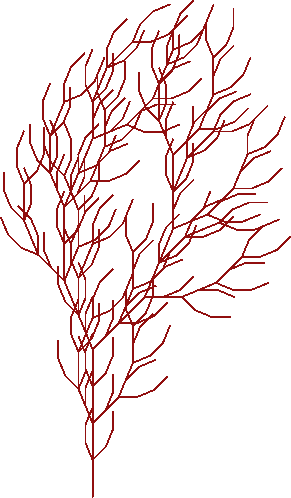
\includegraphics[width=0.33\textwidth]{tree2.png}
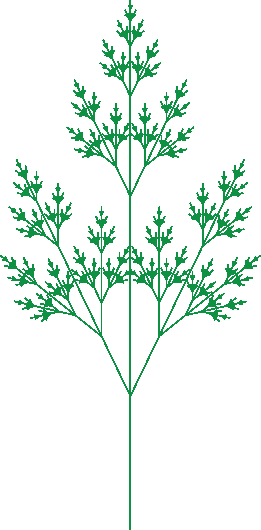
\includegraphics[width=0.28\textwidth]{tree3.png}
\end{center}
\end{frame}

\begin{frame}[fragile]
	\frametitle{Polygonen}
\begin{columns}[c]
\column{0.6\textwidth}
\begin{itemize}
\item Accolades vormen delen die aaneengesloten moeten zijn
\item Elke beweging maakt een driehoek van het beginpunt en de 2 laatste punten.
\pause
\item $F\{-f+f+f-|-f+f+f\}$ $(\sigma = 30^{\circ})$
\end{itemize}
\column{0.4\textwidth}
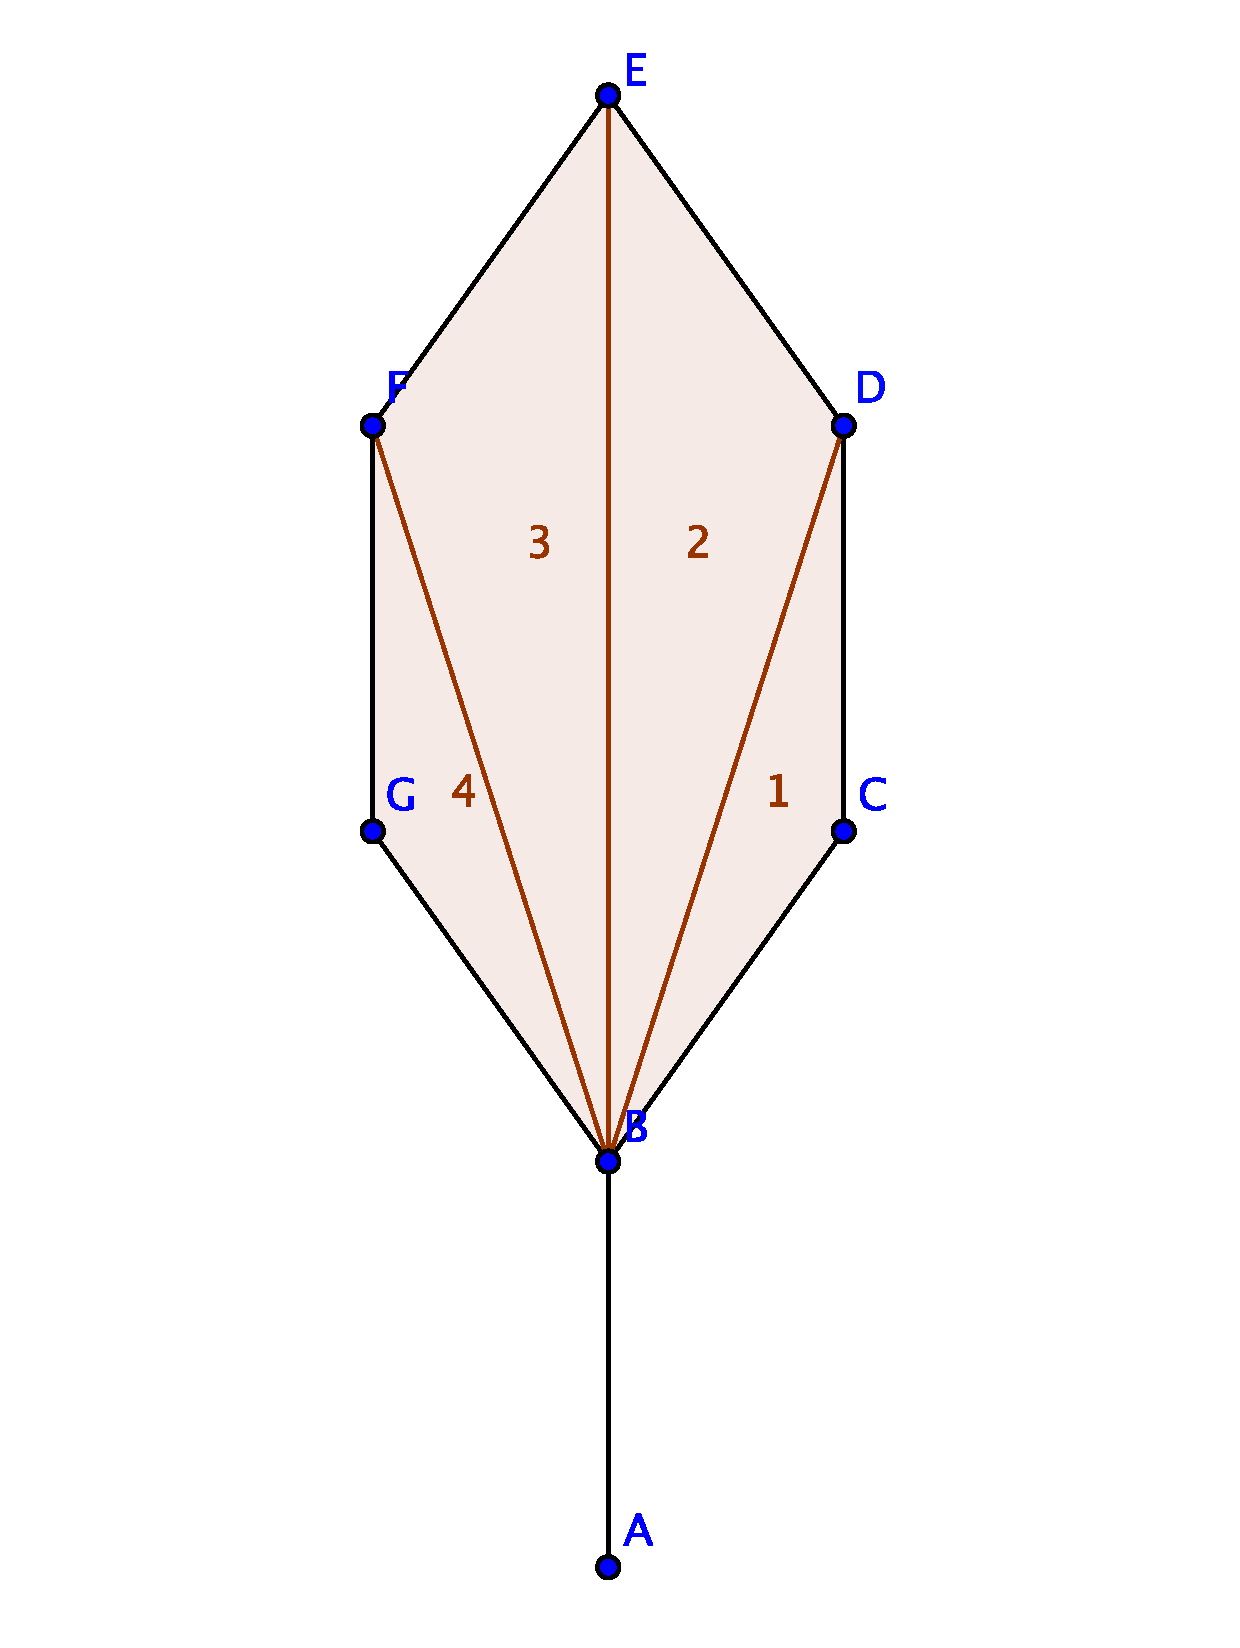
\includegraphics[width=\textwidth]{polygons.pdf}
\end{columns}
\end{frame}


\begin{frame}[fragile]
	\frametitle{}
\begin{center}
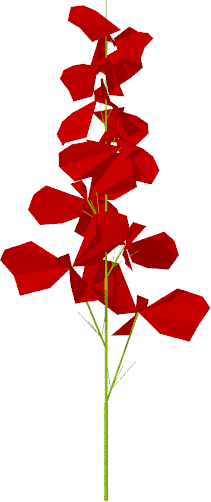
\includegraphics[height=0.8\textheight]{lily_red.png}
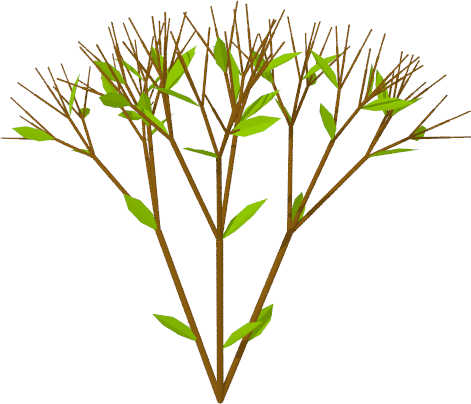
\includegraphics[height=0.8\textheight]{plant6.png}
\end{center}
\end{frame}

\section{Implementatie}

\begin{frame}[fragile]
	\frametitle{Sierpinski triangle}
\begin{columns}[l]
\column{0.6\textwidth}
\begin{itemize}
\item Axiom = $A$
\item $\sigma = 90^{\circ}$
\item Production rules:
	\begin{description}
	\item[A] $\rightarrow B-A-B$
	\item[B] $\rightarrow A+B+A$
	\end{description}
\end{itemize}
\column{0.4\textwidth}
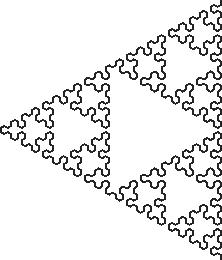
\includegraphics[width=\textwidth]{triangle.png}
\end{columns}
\end{frame}

\subsection{Straight-forward}

\begin{frame}[fragile]
	\frametitle{Straight-forward Implementatie}
\begin{verbatim}
//Given: axiom (string), rules (array of string)
currentstring = axiom
iteration = 0

function iterate()
    newstring = ""
    iteration = iteration + 1
    foreach c in currentstring
        if (c in rules)
            newstring = newstring + rules[c]
        else
            newstring = newstring + c
    currentstring = newstring
\end{verbatim}
\end{frame}

\begin{frame}[fragile]
	\frametitle{Complexiteiten Sierpinski-driehoek}
\begin{itemize}
\item Plaatscomplexiteit: $O(3^I)$
\item Tijdscomplexiteit (opbouw structuur): $O(3^I)$
\item Zowel tijd- als plaatscomplexiteit zijn exponentieel
\end{itemize}
\end{frame}

\subsection{Tree-based}

\begin{frame}[fragile]
	\frametitle{Tree-based structuur}
\begin{itemize}
\item Het axiom is een root-node
\item Elke productie-body + iteratieniveau is een leaf-node
\item Hierin staat pointers naar de verwijzende leaf-nodes op diepere niveau
\end{itemize}
\end{frame}

\begin{frame}[fragile]
	\frametitle{Tree-based structuur}
\begin{center}
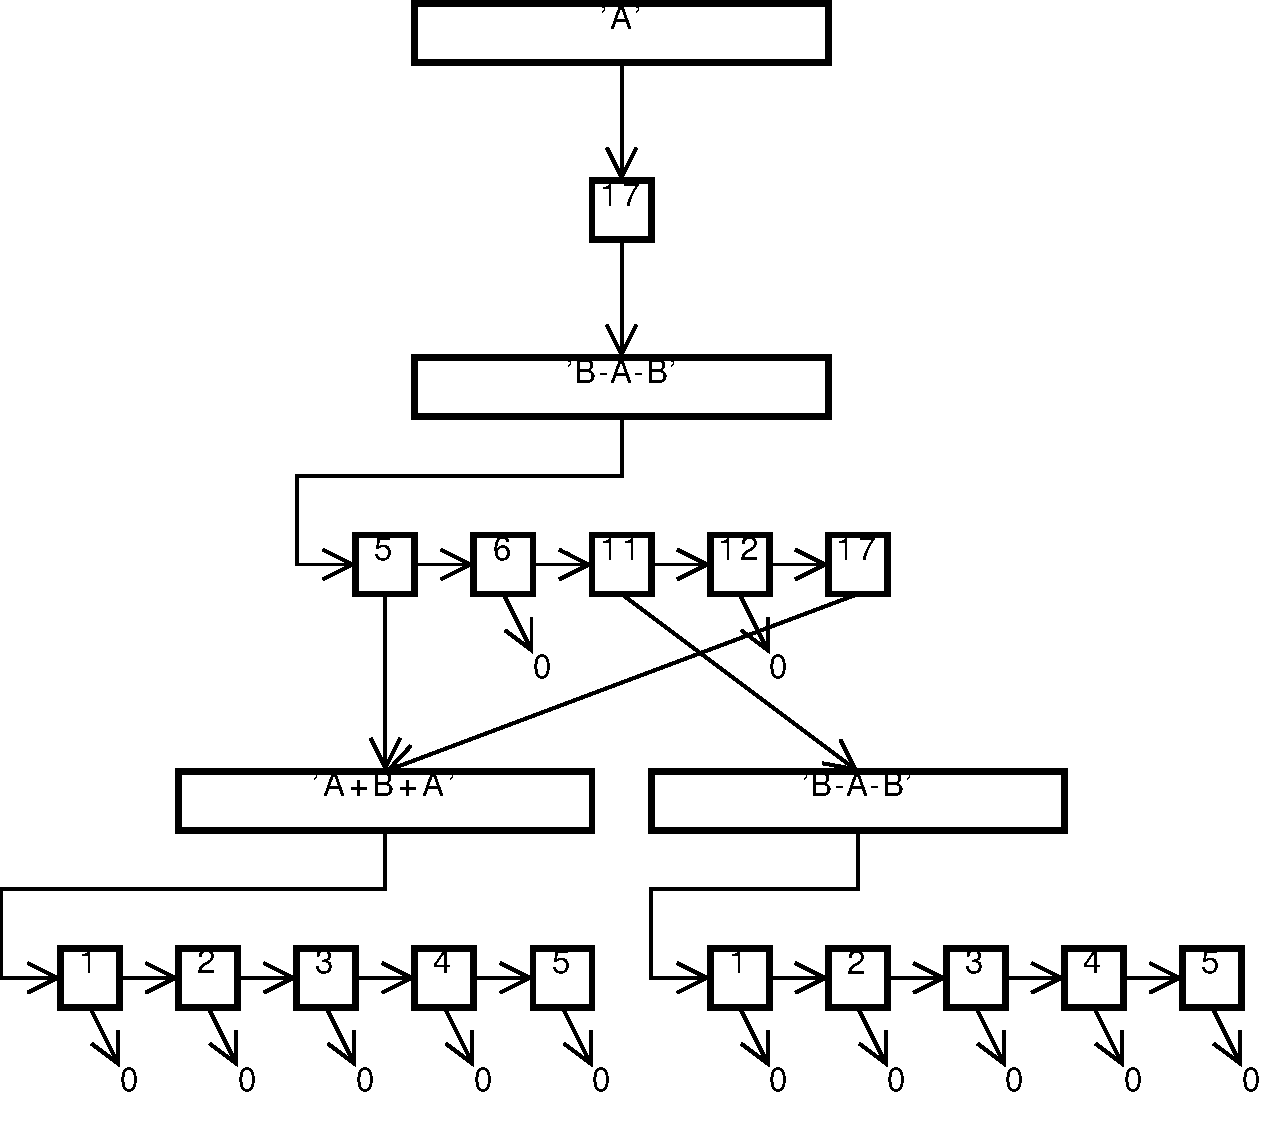
\includegraphics[height=0.9\textheight]{struct.pdf}
\end{center}
\end{frame}


\begin{frame}[fragile]
	\frametitle{Complexiteiten Sierpinski-driehoek}
\begin{itemize}
\item Plaatscomplexiteit: $O(I)$
\item Tijdscomplexiteit* (opbouw structuur): $O(I)$
\pause
\\ *Enkel de tijd voor het opbouwen van de structuur is berekent, een traversal van de tree zal elke karakter moeten opvragen (mbv Binary Search).
\end{itemize}
\end{frame}

\section{Optimalisaties}
\begin{frame}[fragile]
	\frametitle{Optimalisaties voor het tekenen}
\begin{itemize}
\item Turtle graphics gebruiken 1 karakter/actie
\item Parameters lezen is vrij intensief
\end{itemize}
\end{frame}

\begin{frame}[fragile]
	\frametitle{Run-Length Encoding}
\begin{itemize}
\item $++++ \Rightarrow +'4$
\pause
\item Korter
\item Snellere uitvoering
\pause
\item $++--++-+ \Rightarrow +'2$
\pause
\item Speedup: $18-24\%$
\end{itemize}
\end{frame}

\begin{frame}[fragile]
	\frametitle{Parameters inlinen}
\begin{itemize}
\item Parameters=\{\} $F(0.3333)$
\item $\Rightarrow$ Parameters=\{0.3333\} $F*0$
\pause
\item Korter
\item Sneller (niet telkens parsen van een float maar lookup in tabel)
\pause
\item Speedup: $14-21\%$
\end{itemize}
\end{frame}


\end{document}
